\documentclass{beamer}

%
% Common preamble for all three parts.
%

\usepackage{xeCJK}
\setCJKmainfont{TW-Kai.ttf}
\setCJKsansfont{TW-kai.ttf}
\setCJKmonofont{TW-kai.ttf}

\usepackage[english]{babel}
\usepackage{amsmath}
\usepackage{color}
\usepackage[cache=false]{minted}
\usepackage{hyperref}
\usepackage{multicol}
\usepackage{tabularx}
\usepackage{tikz}

% only inline todonotes work
\usepackage{xkeyval}
\usepackage[textsize=small]{todonotes}
\presetkeys{todonotes}{inline}{}

\usetikzlibrary{shapes,arrows,positioning,shadows}

% no nav buttons
\usenavigationsymbolstemplate{}

\newcommand{\bftt}[1]{\textbf{\texttt{#1}}}
\newcommand{\comment}[1]{{\color[HTML]{008080}\textit{\textbf{\texttt{#1}}}}}
\newcommand{\cmd}[1]{{\color[HTML]{008000}\bftt{#1}}}
\newcommand{\bs}{\char`\\}
\newcommand{\cmdbs}[1]{\cmd{\bs#1}}
\newcommand{\lcb}{\char '173}
\newcommand{\rcb}{\char '175}
\newcommand{\cmdbegin}[1]{\cmdbs{begin\lcb}\bftt{#1}\cmd{\rcb}}
\newcommand{\cmdend}[1]{\cmdbs{end\lcb}\bftt{#1}\cmd{\rcb}}

\newcommand{\wllogo}{\textbf{Overleaf}}

% this is where the example source files are loaded from
% do not include a trailing slash
\newcommand{\fileuri}{https://raw.github.com/jdleesmiller/latex-course/master/en}

\newcommand{\wlserver}{https://www.overleaf.com}
\newcommand{\wlnewdoc}[1]{\wlserver/docs?snip\_uri=\fileuri/#1\&splash=none}

\def\tikzname{Ti\emph{k}Z}

% from http://tex.stackexchange.com/questions/5226/keyboard-font-for-latex
\newcommand*\keystroke[1]{%
  \tikz[baseline=(key.base)]
    \node[%
      draw,
      fill=white,
      drop shadow={shadow xshift=0.25ex,shadow yshift=-0.25ex,fill=black,opacity=0.75},
      rectangle,
      rounded corners=2pt,
      inner sep=1pt,
      line width=0.5pt,
      font=\scriptsize\sffamily
    ](key) {#1\strut}
  ;
}
\newcommand{\keystrokebftt}[1]{\keystroke{\bftt{#1}}}

% stolen from minted.dtx
\newenvironment{exampletwoup}
  {\VerbatimEnvironment
   \begin{VerbatimOut}{example.out}}
  {\end{VerbatimOut}
   \setlength{\parindent}{0pt}
   \fbox{\begin{tabular}{l|l}
   \begin{minipage}{0.55\linewidth}
     \inputminted[fontsize=\small,resetmargins]{latex}{example.out}
   \end{minipage} &
   \begin{minipage}{0.35\linewidth}
     \input{example.out}
   \end{minipage}
   \end{tabular}}}

\newenvironment{exampletwouptiny}
  {\VerbatimEnvironment
   \begin{VerbatimOut}{example.out}}
  {\end{VerbatimOut}
   \setlength{\parindent}{0pt}
   \fbox{\begin{tabular}{l|l}
   \begin{minipage}{0.55\linewidth}
     \inputminted[fontsize=\scriptsize,resetmargins]{latex}{example.out}
   \end{minipage} &
   \begin{minipage}{0.35\linewidth}
     \setlength{\parskip}{6pt plus 1pt minus 1pt}%
     \raggedright\scriptsize\input{example.out}
   \end{minipage}
   \end{tabular}}}

\newenvironment{exampletwouptinynoframe}
  {\VerbatimEnvironment
   \begin{VerbatimOut}{example.out}}
  {\end{VerbatimOut}
   \setlength{\parindent}{0pt}
   \begin{tabular}{l|l}
   \begin{minipage}{0.55\linewidth}
     \inputminted[fontsize=\scriptsize,resetmargins]{latex}{example.out}
   \end{minipage} &
   \begin{minipage}{0.35\linewidth}
     \setlength{\parskip}{6pt plus 1pt minus 1pt}%
     \raggedright\scriptsize\input{example.out}
   \end{minipage}
   \end{tabular}}

\title{一份互動式的\LaTeX\ 介紹}
\author{作者:Dr John D. Lees-Miller \texorpdfstring{\\[2mm]}{}
\small{譯者:周造麟}}
\titlegraphic{%

\includegraphics[height=36pt]{overleaf}\\[1em]

\includegraphics[height=24pt]{UoB-logo}
}


\subtitle{第二部:有結構的文件與更多}

\begin{document}

%%%%%%%%%%%%%%%%%%%%%%%%%%%%%%%%%%%%%%%%%%%%%%%%%%%%%%%%%%%%%%%%%%%%%%%%%%%%%%%
%%%%%%%%%%%%%%%%%%%%%%%%%%%%%%%%%%%%%%%%%%%%%%%%%%%%%%%%%%%%%%%%%%%%%%%%%%%%%%%
%%%%%%%%%%%%%%%%%%%%%%%%%%%%%%%%%%%%%%%%%%%%%%%%%%%%%%%%%%%%%%%%%%%%%%%%%%%%%%%
\begin{frame}
\titlepage
\end{frame}

%%%%%%%%%%%%%%%%%%%%%%%%%%%%%%%%%%%%%%%%%%%%%%%%%%%%%%%%%%%%%%%%%%%%%%%%%%%%%%%
%%%%%%%%%%%%%%%%%%%%%%%%%%%%%%%%%%%%%%%%%%%%%%%%%%%%%%%%%%%%%%%%%%%%%%%%%%%%%%%
%%%%%%%%%%%%%%%%%%%%%%%%%%%%%%%%%%%%%%%%%%%%%%%%%%%%%%%%%%%%%%%%%%%%%%%%%%%%%%%
\section{結構化文件}

%%%%%%%%%%%%%%%%%%%%%%%%%%%%%%%%%%%%%%%%%%%%%%%%%%%%%%%%%%%%%%%%%%%%%%%%%%%%%%%
%%%%%%%%%%%%%%%%%%%%%%%%%%%%%%%%%%%%%%%%%%%%%%%%%%%%%%%%%%%%%%%%%%%%%%%%%%%%%%%
%%%%%%%%%%%%%%%%%%%%%%%%%%%%%%%%%%%%%%%%%%%%%%%%%%%%%%%%%%%%%%%%%%%%%%%%%%%%%%%
\begin{frame}{大綱}
\begin{multicols}{2}
\tableofcontents[currentsection]
\end{multicols}
\end{frame}

%%%%%%%%%%%%%%%%%%%%%%%%%%%%%%%%%%%%%%%%%%%%%%%%%%%%%%%%%%%%%%%%%%%%%%%%%%%%%%%
%%%%%%%%%%%%%%%%%%%%%%%%%%%%%%%%%%%%%%%%%%%%%%%%%%%%%%%%%%%%%%%%%%%%%%%%%%%%%%%
%%%%%%%%%%%%%%%%%%%%%%%%%%%%%%%%%%%%%%%%%%%%%%%%%%%%%%%%%%%%%%%%%%%%%%%%%%%%%%%
\begin{frame}{\insertsection}
\begin{itemize}
\item 在第一部我們學了用來排版文字和數學方程式的命令與環境
\item 現在我們將會探討結構化文件的命令與環境
\item 你可以在Overleaf中嘗試這些新的命令
\end{itemize}
\vskip 2em
\begin{center}
\fbox{\href{\wlnewdoc{basics.tex}}{%
點擊這裡以在\wllogo{}中打開範例文件}}
\\[1ex]\scriptsize{}
為得到最好的使用體驗,推薦使用 \href{http://www.google.com/chrome}{Google Chrome} 或 \href{http://www.mozilla.org/en-US/firefox/new/}{FireFox}
\end{center}
\vskip 2ex
\begin{itemize}
\item 讓我們開始吧!
\end{itemize}
\end{frame}

%%%%%%%%%%%%%%%%%%%%%%%%%%%%%%%%%%%%%%%%%%%%%%%%%%%%%%%%%%%%%%%%%%%%%%%%%%%%%%%
%%%%%%%%%%%%%%%%%%%%%%%%%%%%%%%%%%%%%%%%%%%%%%%%%%%%%%%%%%%%%%%%%%%%%%%%%%%%%%%
%%%%%%%%%%%%%%%%%%%%%%%%%%%%%%%%%%%%%%%%%%%%%%%%%%%%%%%%%%%%%%%%%%%%%%%%%%%%%%%
\subsection{標題與摘要}
\begin{frame}[fragile]{\insertsubsection}
\begin{itemize}{\small
\item 在導言區告訴\LaTeX{}標題(\cmdbs{title})和作者名(\cmdbs{author})
\item 然後使用在文件中使用\cmdbs{maketitle}製造標題
\item 使用\bftt{abstract}環境建立摘要
}\end{itemize}
\begin{minipage}{0.55\linewidth}
\inputminted[fontsize=\scriptsize,frame=single,resetmargins]{latex}%
  {structure-title.tex}
\end{minipage}
\begin{minipage}{0.35\linewidth}

\includegraphics[width=\textwidth,clip,trim=2.2in 7in 2.2in 2in]{structure-title.pdf}
\end{minipage}
\end{frame}

%%%%%%%%%%%%%%%%%%%%%%%%%%%%%%%%%%%%%%%%%%%%%%%%%%%%%%%%%%%%%%%%%%%%%%%%%%%%%%%
%%%%%%%%%%%%%%%%%%%%%%%%%%%%%%%%%%%%%%%%%%%%%%%%%%%%%%%%%%%%%%%%%%%%%%%%%%%%%%%
%%%%%%%%%%%%%%%%%%%%%%%%%%%%%%%%%%%%%%%%%%%%%%%%%%%%%%%%%%%%%%%%%%%%%%%%%%%%%%%
\subsection{節與小節}
\begin{frame}{\insertsubsection}
\begin{itemize}{\small
\item 使用\cmdbs{section}製造節,使用\cmdbs{subsection}製造小節
\item 你可以猜猜\cmdbs{section*}和\cmdbs{subsection*}是做什麼的嗎?
}\end{itemize}
\begin{minipage}{0.55\linewidth}
\inputminted[fontsize=\scriptsize,frame=single,resetmargins]{latex}%
  {structure-sections.tex}
\end{minipage}
\begin{minipage}{0.35\linewidth}
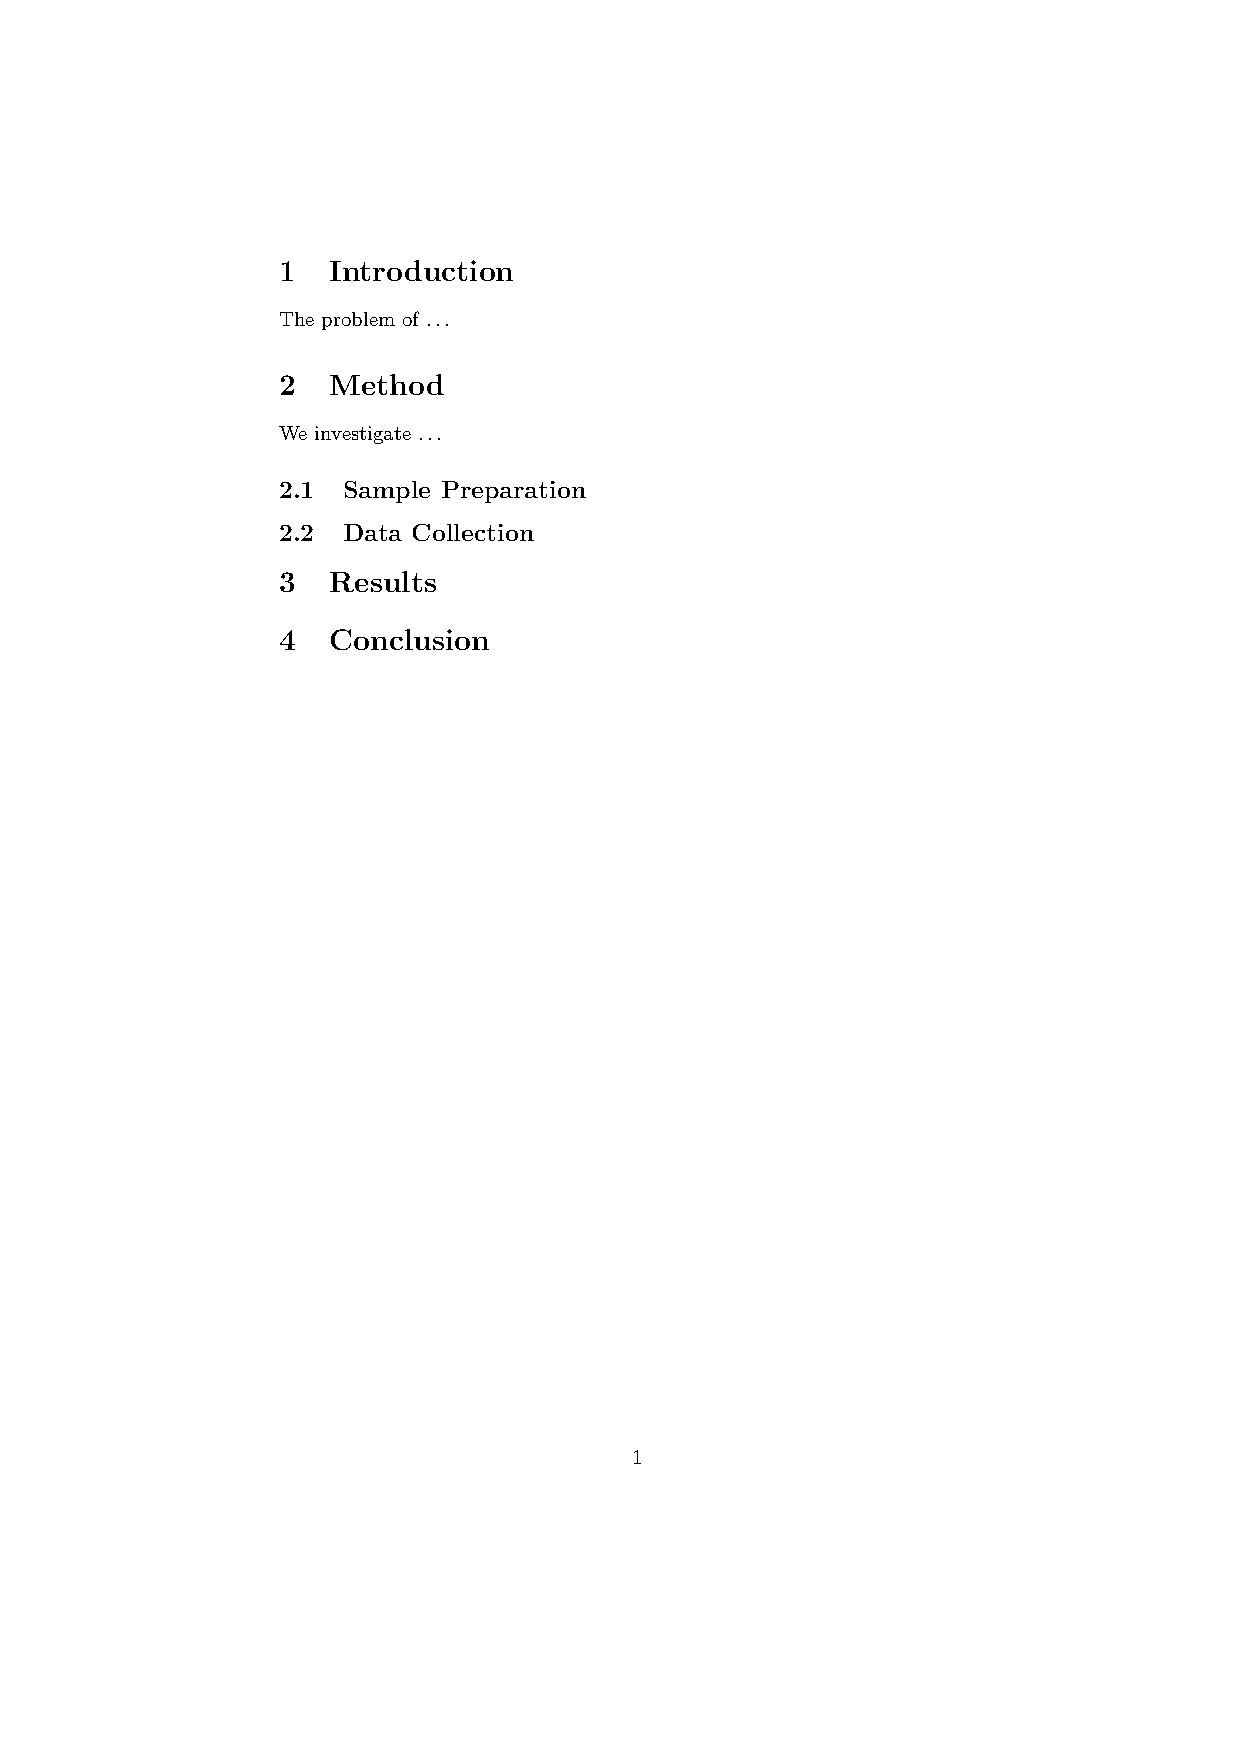
\includegraphics[width=\textwidth,clip,trim=1.5in 6in 4in 1in]{structure-sections.pdf}
\end{minipage}
\end{frame}

%%%%%%%%%%%%%%%%%%%%%%%%%%%%%%%%%%%%%%%%%%%%%%%%%%%%%%%%%%%%%%%%%%%%%%%%%%%%%%%
%%%%%%%%%%%%%%%%%%%%%%%%%%%%%%%%%%%%%%%%%%%%%%%%%%%%%%%%%%%%%%%%%%%%%%%%%%%%%%%
%%%%%%%%%%%%%%%%%%%%%%%%%%%%%%%%%%%%%%%%%%%%%%%%%%%%%%%%%%%%%%%%%%%%%%%%%%%%%%%
\subsection{標籤與交叉引用}
\begin{frame}[fragile]{\insertsubsection}
\begin{itemize}{\small
\item 使用\cmdbs{label}創造標籤,使用\cmdbs{ref}以自動獲取標籤所在的頁數
\item \bftt{amsmath} package提供為提供\cmdbs{eqref}來引用方程式
}\end{itemize}
\begin{minipage}{0.55\linewidth}
\inputminted[fontsize=\scriptsize,frame=single,resetmargins]{latex}%
  {structure-crossref.tex}
\end{minipage}
\begin{minipage}{0.35\linewidth}
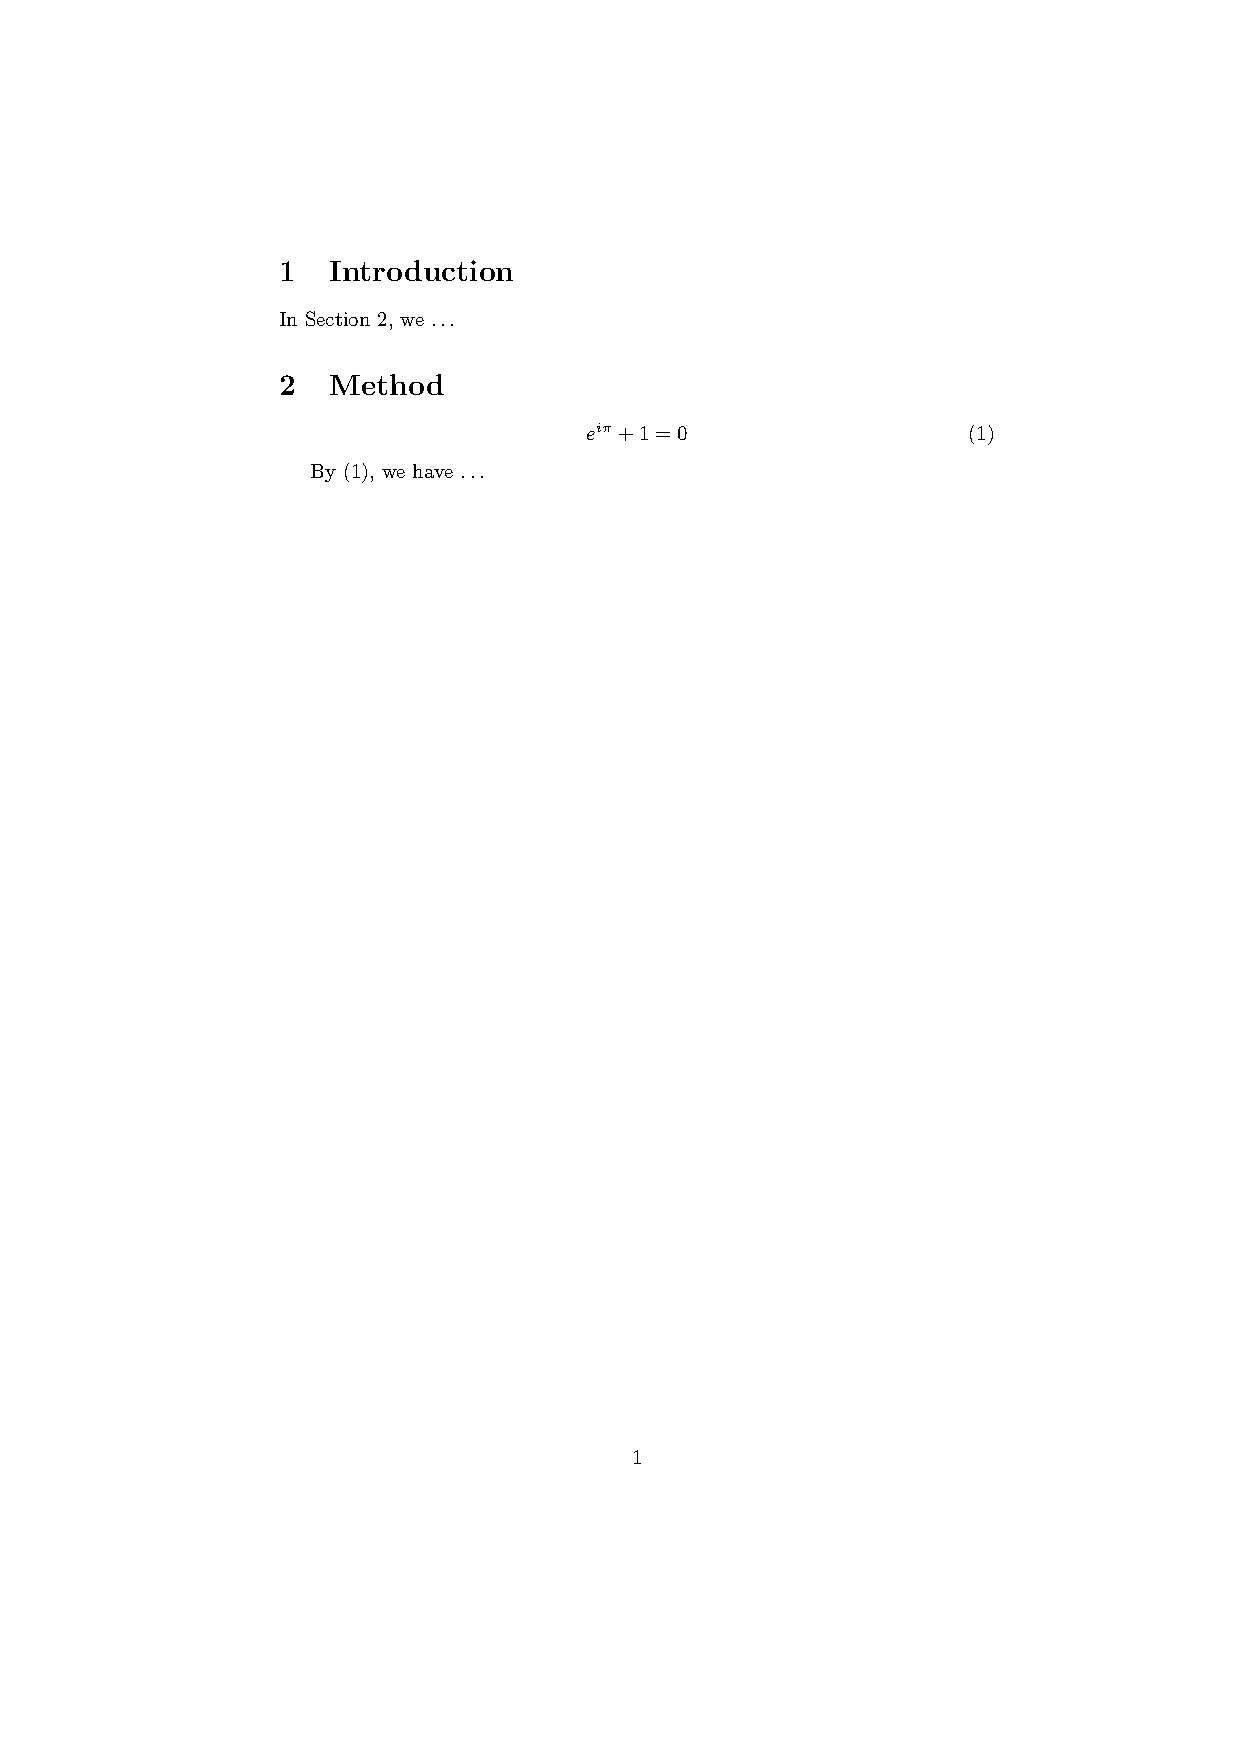
\includegraphics[width=\textwidth,clip,trim=1.8in 6in 1.6in 1in]{structure-crossref.pdf}
\end{minipage}
\end{frame}

%%%%%%%%%%%%%%%%%%%%%%%%%%%%%%%%%%%%%%%%%%%%%%%%%%%%%%%%%%%%%%%%%%%%%%%%%%%%%%%
%%%%%%%%%%%%%%%%%%%%%%%%%%%%%%%%%%%%%%%%%%%%%%%%%%%%%%%%%%%%%%%%%%%%%%%%%%%%%%%
%%%%%%%%%%%%%%%%%%%%%%%%%%%%%%%%%%%%%%%%%%%%%%%%%%%%%%%%%%%%%%%%%%%%%%%%%%%%%%%
\subsection{小試身手}
\begin{frame}[fragile]{結構化文件練習}

\begin{block}{嘗試利用\LaTeX\ 為這份短文排版:
\footnote{來自 \url{http://pdos.csail.mit.edu/scigen/}一個隨機文件產生器}}
\begin{center}
\fbox{\href{\fileuri/structure-exercise-solution.pdf}{%
點擊這裡開啟範例}}
\end{center}
讓你的文件看起來像範例,使用\cmdbs{ref}和\cmdbs{eqref} 來避免明確地將編號寫進文件中
\end{block}
\vskip 2ex
\begin{center}
\fbox{\href{\wlnewdoc{structure-exercise.tex}}{%
點擊以在\wllogo{}中開啟}}
\end{center}

\begin{itemize}
\item 嘗試完之後
\fbox{\href{\wlnewdoc{structure-exercise-solution.tex}}{%
點擊這裡來看解答}}.
\end{itemize}
\end{frame}

%%%%%%%%%%%%%%%%%%%%%%%%%%%%%%%%%%%%%%%%%%%%%%%%%%%%%%%%%%%%%%%%%%%%%%%%%%%%%%%
%%%%%%%%%%%%%%%%%%%%%%%%%%%%%%%%%%%%%%%%%%%%%%%%%%%%%%%%%%%%%%%%%%%%%%%%%%%%%%%
%%%%%%%%%%%%%%%%%%%%%%%%%%%%%%%%%%%%%%%%%%%%%%%%%%%%%%%%%%%%%%%%%%%%%%%%%%%%%%%
\section{圖片與表格}

%%%%%%%%%%%%%%%%%%%%%%%%%%%%%%%%%%%%%%%%%%%%%%%%%%%%%%%%%%%%%%%%%%%%%%%%%%%%%%%
%%%%%%%%%%%%%%%%%%%%%%%%%%%%%%%%%%%%%%%%%%%%%%%%%%%%%%%%%%%%%%%%%%%%%%%%%%%%%%%
%%%%%%%%%%%%%%%%%%%%%%%%%%%%%%%%%%%%%%%%%%%%%%%%%%%%%%%%%%%%%%%%%%%%%%%%%%%%%%%
\begin{frame}{大綱}
\begin{multicols}{2}
\tableofcontents[currentsection]
\end{multicols}
\end{frame}

%%%%%%%%%%%%%%%%%%%%%%%%%%%%%%%%%%%%%%%%%%%%%%%%%%%%%%%%%%%%%%%%%%%%%%%%%%%%%%%
%%%%%%%%%%%%%%%%%%%%%%%%%%%%%%%%%%%%%%%%%%%%%%%%%%%%%%%%%%%%%%%%%%%%%%%%%%%%%%%
%%%%%%%%%%%%%%%%%%%%%%%%%%%%%%%%%%%%%%%%%%%%%%%%%%%%%%%%%%%%%%%%%%%%%%%%%%%%%%%
\subsection{圖片}
\begin{frame}[fragile]{\insertsubsection{}:graphicx}
\begin{itemize}
\item 需使用\bftt{graphicx} package提供的\cmdbs{includegraphics}命令
\item 支援的圖片格式有 JPEG, PNG 和 PDF (通常)
\end{itemize}
\begin{exampletwouptiny}

\includegraphics[
  width=0.5\textwidth]{gerbil}


\includegraphics[
  width=0.3\textwidth,
  angle=270]{gerbil}
\end{exampletwouptiny}

\tiny{Image license: \href{https://pixabay.com/en/animal-apple-attractive-beautiful-1239390/}{CC0}}
\end{frame}

%%%%%%%%%%%%%%%%%%%%%%%%%%%%%%%%%%%%%%%%%%%%%%%%%%%%%%%%%%%%%%%%%%%%%%%%%%%%%%%
%%%%%%%%%%%%%%%%%%%%%%%%%%%%%%%%%%%%%%%%%%%%%%%%%%%%%%%%%%%%%%%%%%%%%%%%%%%%%%%
%%%%%%%%%%%%%%%%%%%%%%%%%%%%%%%%%%%%%%%%%%%%%%%%%%%%%%%%%%%%%%%%%%%%%%%%%%%%%%%
\begin{frame}[fragile]{小插曲:可選參數}
\begin{itemize}
\item 我們使用中括號來指定可選參數\keystrokebftt{[} \keystrokebftt{]}而不是使用花括號\keystrokebftt{\{} \keystrokebftt{\}}.
\item \cmdbs{includegraphics}接受一些調整圖片的可選參數,舉個例子:\bftt{width=0.3\cmdbs{textwidth}}將圖片寬度設為周遭文字(\cmdbs{textwidth}).的30\%
\item \cmdbs{documentclass}同樣接受可選參數
\mint{latex}|\documentclass[12pt,twocolumn]{article}|
\vskip 3ex
加大文字大小(12pt)和開啟了雙欄模式
\item 哪裡可以找到更多資訊?投影片的做後有連結!
\end{itemize}
\end{frame}

%%%%%%%%%%%%%%%%%%%%%%%%%%%%%%%%%%%%%%%%%%%%%%%%%%%%%%%%%%%%%%%%%%%%%%%%%%%%%%%
%%%%%%%%%%%%%%%%%%%%%%%%%%%%%%%%%%%%%%%%%%%%%%%%%%%%%%%%%%%%%%%%%%%%%%%%%%%%%%%
%%%%%%%%%%%%%%%%%%%%%%%%%%%%%%%%%%%%%%%%%%%%%%%%%%%%%%%%%%%%%%%%%%%%%%%%%%%%%%%
\subsection[fragile]{浮動體}
\begin{frame}{\insertsubsection}
\begin{itemize}
\item 讓\LaTeX{}決定圖片的具體位置(圖片可以``浮動'').
\item 你可以給圖片加上一段能被\cmdbs{ref}引用的說明文字
\end{itemize}
\begin{minipage}{0.55\linewidth}
\inputminted[fontsize=\scriptsize,frame=single,resetmargins]{latex}%
  {media-graphics.tex}
\end{minipage}
\begin{minipage}{0.35\linewidth}
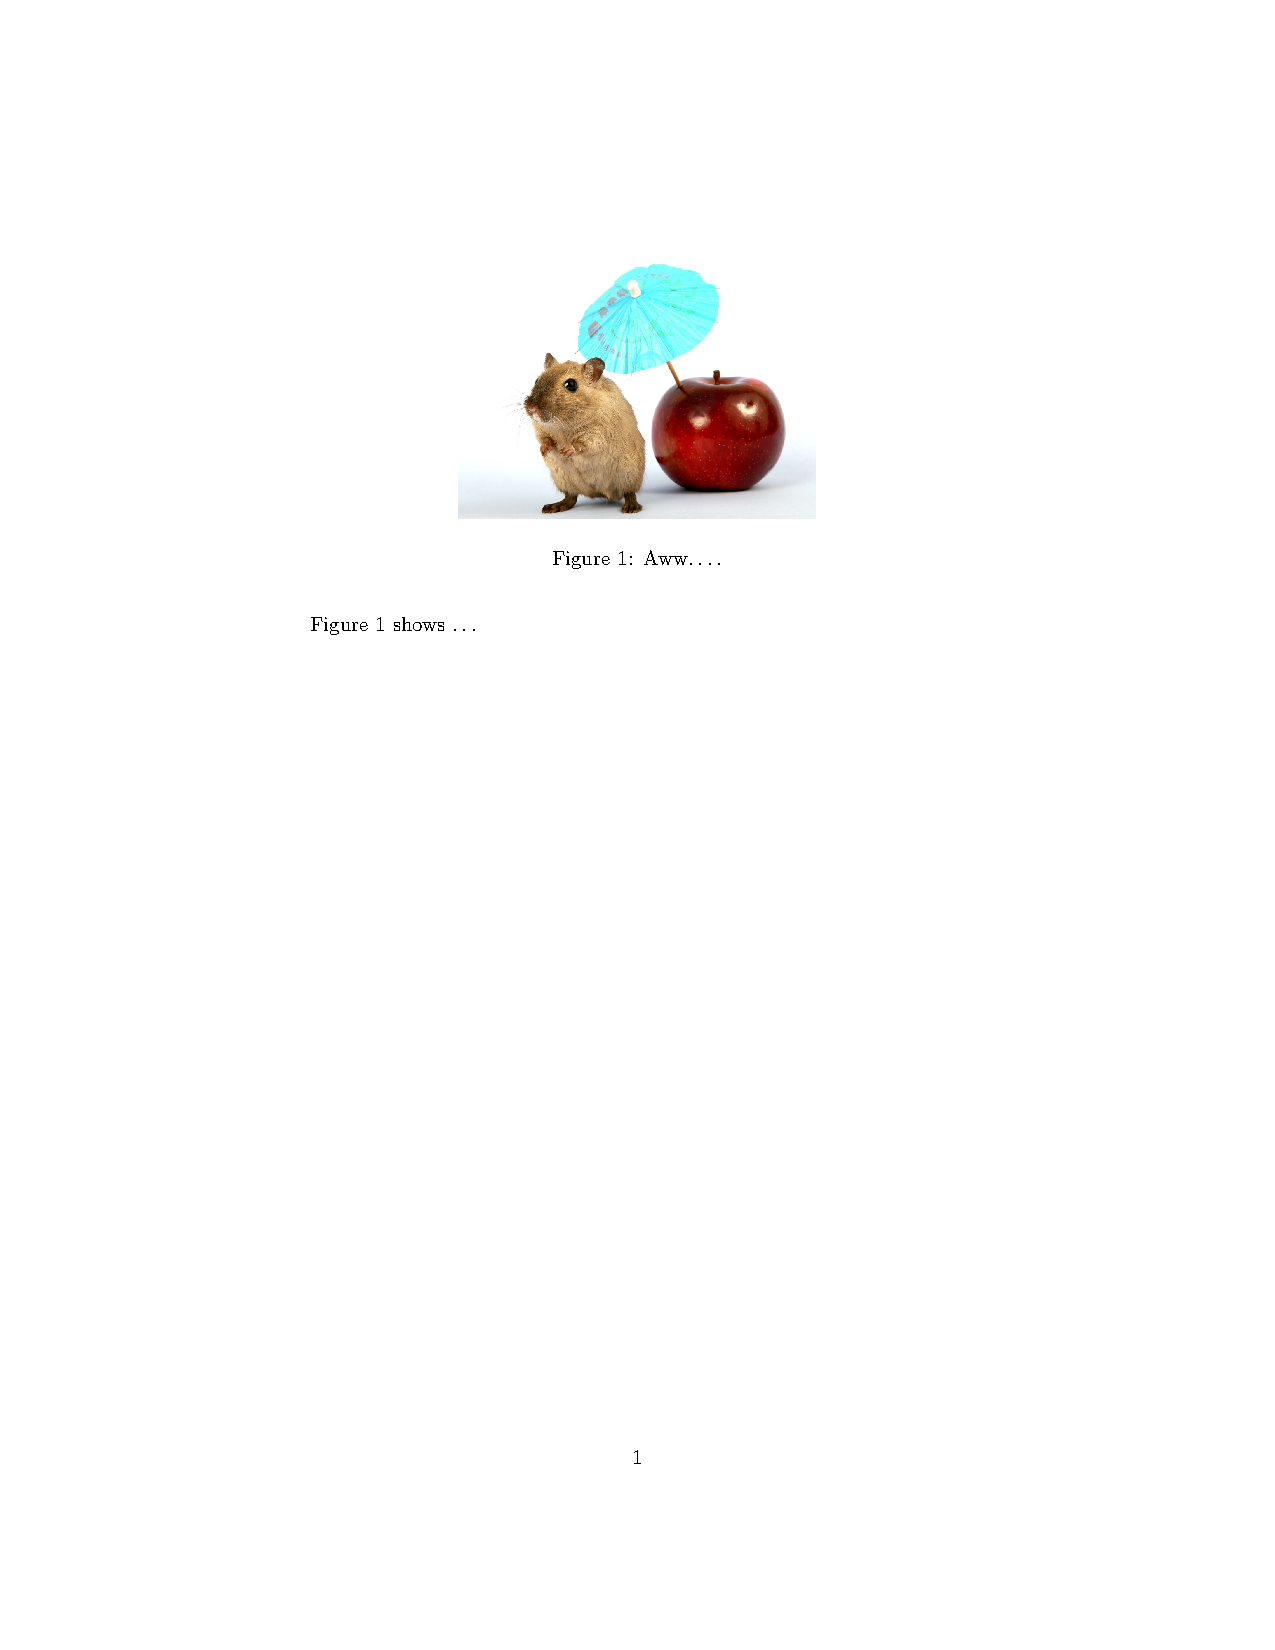
\includegraphics[width=\textwidth,clip,trim=2in 5in 3in 1in]{media-graphics.pdf}
\end{minipage}

\tiny{Image license: \href{https://pixabay.com/en/animal-apple-attractive-beautiful-1239390/}{CC0}}
\end{frame}

%%%%%%%%%%%%%%%%%%%%%%%%%%%%%%%%%%%%%%%%%%%%%%%%%%%%%%%%%%%%%%%%%%%%%%%%%%%%%%%
%%%%%%%%%%%%%%%%%%%%%%%%%%%%%%%%%%%%%%%%%%%%%%%%%%%%%%%%%%%%%%%%%%%%%%%%%%%%%%%
%%%%%%%%%%%%%%%%%%%%%%%%%%%%%%%%%%%%%%%%%%%%%%%%%%%%%%%%%%%%%%%%%%%%%%%%%%%%%%%
\subsection{表格}
\begin{frame}[fragile]{\insertsubsection}
\begin{itemize}
\item 在\LaTeX{}中使用表格需經過一番適應
\item 使用\bftt{tabularx} package 提供的\bftt{tabular}環境
\item 指定表格靠齊位置的參數 --- \textbf{l}eft, \textbf{r}ight, \textbf{r}ight
\begin{exampletwouptiny}
\begin{tabular}{lrr}
Item   & Qty & Unit \$ \\
Widget & 1   & 199.99  \\
Gadget & 2   & 399.99  \\
Cable  & 3   & 19.99   \\
\end{tabular}
\end{exampletwouptiny}
\item 這同時也可以指定表格中的垂直線,使用\cmdbs{hline}命令指定水平線
\begin{exampletwouptiny}
\begin{tabular}{|l|r|r|} \hline
Item   & Qty & Unit \$ \\\hline
Widget & 1   & 199.99  \\
Gadget & 2   & 399.99  \\
Cable  & 3   & 19.99   \\\hline
\end{tabular}
\end{exampletwouptiny}
\item 使用與號\keystrokebftt{\&}來接每一格分開,使用雙重反斜槓\keystrokebftt{\bs}\keystrokebftt{\bs}來換行(就像 part 1 中提過的\bftt{align*}環境)
\end{itemize}
\end{frame}

%%%%%%%%%%%%%%%%%%%%%%%%%%%%%%%%%%%%%%%%%%%%%%%%%%%%%%%%%%%%%%%%%%%%%%%%%%%%%%%
%%%%%%%%%%%%%%%%%%%%%%%%%%%%%%%%%%%%%%%%%%%%%%%%%%%%%%%%%%%%%%%%%%%%%%%%%%%%%%%
%%%%%%%%%%%%%%%%%%%%%%%%%%%%%%%%%%%%%%%%%%%%%%%%%%%%%%%%%%%%%%%%%%%%%%%%%%%%%%%
\addtocontents{toc}{\newpage}
\section{參考書目}

%%%%%%%%%%%%%%%%%%%%%%%%%%%%%%%%%%%%%%%%%%%%%%%%%%%%%%%%%%%%%%%%%%%%%%%%%%%%%%%
%%%%%%%%%%%%%%%%%%%%%%%%%%%%%%%%%%%%%%%%%%%%%%%%%%%%%%%%%%%%%%%%%%%%%%%%%%%%%%%
%%%%%%%%%%%%%%%%%%%%%%%%%%%%%%%%%%%%%%%%%%%%%%%%%%%%%%%%%%%%%%%%%%%%%%%%%%%%%%%
\begin{frame}{大綱}
\begin{multicols}{2}
\tableofcontents[currentsection]
\end{multicols}
\end{frame}

%%%%%%%%%%%%%%%%%%%%%%%%%%%%%%%%%%%%%%%%%%%%%%%%%%%%%%%%%%%%%%%%%%%%%%%%%%%%%%%
%%%%%%%%%%%%%%%%%%%%%%%%%%%%%%%%%%%%%%%%%%%%%%%%%%%%%%%%%%%%%%%%%%%%%%%%%%%%%%%
%%%%%%%%%%%%%%%%%%%%%%%%%%%%%%%%%%%%%%%%%%%%%%%%%%%%%%%%%%%%%%%%%%%%%%%%%%%%%%%
\subsection{bib\TeX}
\begin{frame}[fragile]{\insertsubsection{} 1}
\begin{itemize}
\item 將你的引用資料遵循`bibtex'的格式寫在\bftt{.bib}檔中
\inputminted[fontsize=\scriptsize,frame=single]{latex}{bib-example.bib}
\item 大部分的引用資料管理器可輸出符合`bibtex'格式的檔案
\end{itemize}
\end{frame}

%%%%%%%%%%%%%%%%%%%%%%%%%%%%%%%%%%%%%%%%%%%%%%%%%%%%%%%%%%%%%%%%%%%%%%%%%%%%%%%
%%%%%%%%%%%%%%%%%%%%%%%%%%%%%%%%%%%%%%%%%%%%%%%%%%%%%%%%%%%%%%%%%%%%%%%%%%%%%%%
%%%%%%%%%%%%%%%%%%%%%%%%%%%%%%%%%%%%%%%%%%%%%%%%%%%%%%%%%%%%%%%%%%%%%%%%%%%%%%%
\begin{frame}[fragile]{\insertsubsection{} 2}
\begin{itemize}
\item 在\bftt{.bib}檔中的每一個條目都會有一個\emph{key}來讓你在文件中引用,舉個例子\bftt{Jacobson1999Towards}是這篇這篇文章的key:
\begin{minted}[fontsize=\small,frame=single]{latex}
@Article{Jacobson1999Towards,
  author = {Van Jacobson},
  ...
}
\end{minted}
\item 將key設為作者名加出版年份與標題是個好主意
\item \LaTeX{}可以自動格式化你的行內引文,然後甚至創造出一份引用資料的列表,\LaTeX{}知道最標準的格式,你也可以自行設計
\end{itemize}
\end{frame}

%%%%%%%%%%%%%%%%%%%%%%%%%%%%%%%%%%%%%%%%%%%%%%%%%%%%%%%%%%%%%%%%%%%%%%%%%%%%%%%
%%%%%%%%%%%%%%%%%%%%%%%%%%%%%%%%%%%%%%%%%%%%%%%%%%%%%%%%%%%%%%%%%%%%%%%%%%%%%%%
%%%%%%%%%%%%%%%%%%%%%%%%%%%%%%%%%%%%%%%%%%%%%%%%%%%%%%%%%%%%%%%%%%%%%%%%%%%%%%%
\begin{frame}[fragile]{\insertsubsection{} 3}
\begin{itemize}
\item 使用\bftt{natbib} package\footnote{這裡有一個較新的 package \bftt{biblatex} 提供了更多了功能,但大部分的期刊與模板依舊使\bftt{natbib}.} 提供的\cmdbs{citet} 與 \cmdbs{citep}命令
\item 在文章的最後引用\cmdbs{bibliography},利用\cmdbs{bibliographystyle}來指定格式
\end{itemize}
\begin{minipage}{0.55\linewidth}
\inputminted[fontsize=\scriptsize,frame=single,resetmargins]{latex}%
  {bib-example.tex}
\end{minipage}
\begin{minipage}{0.35\linewidth}
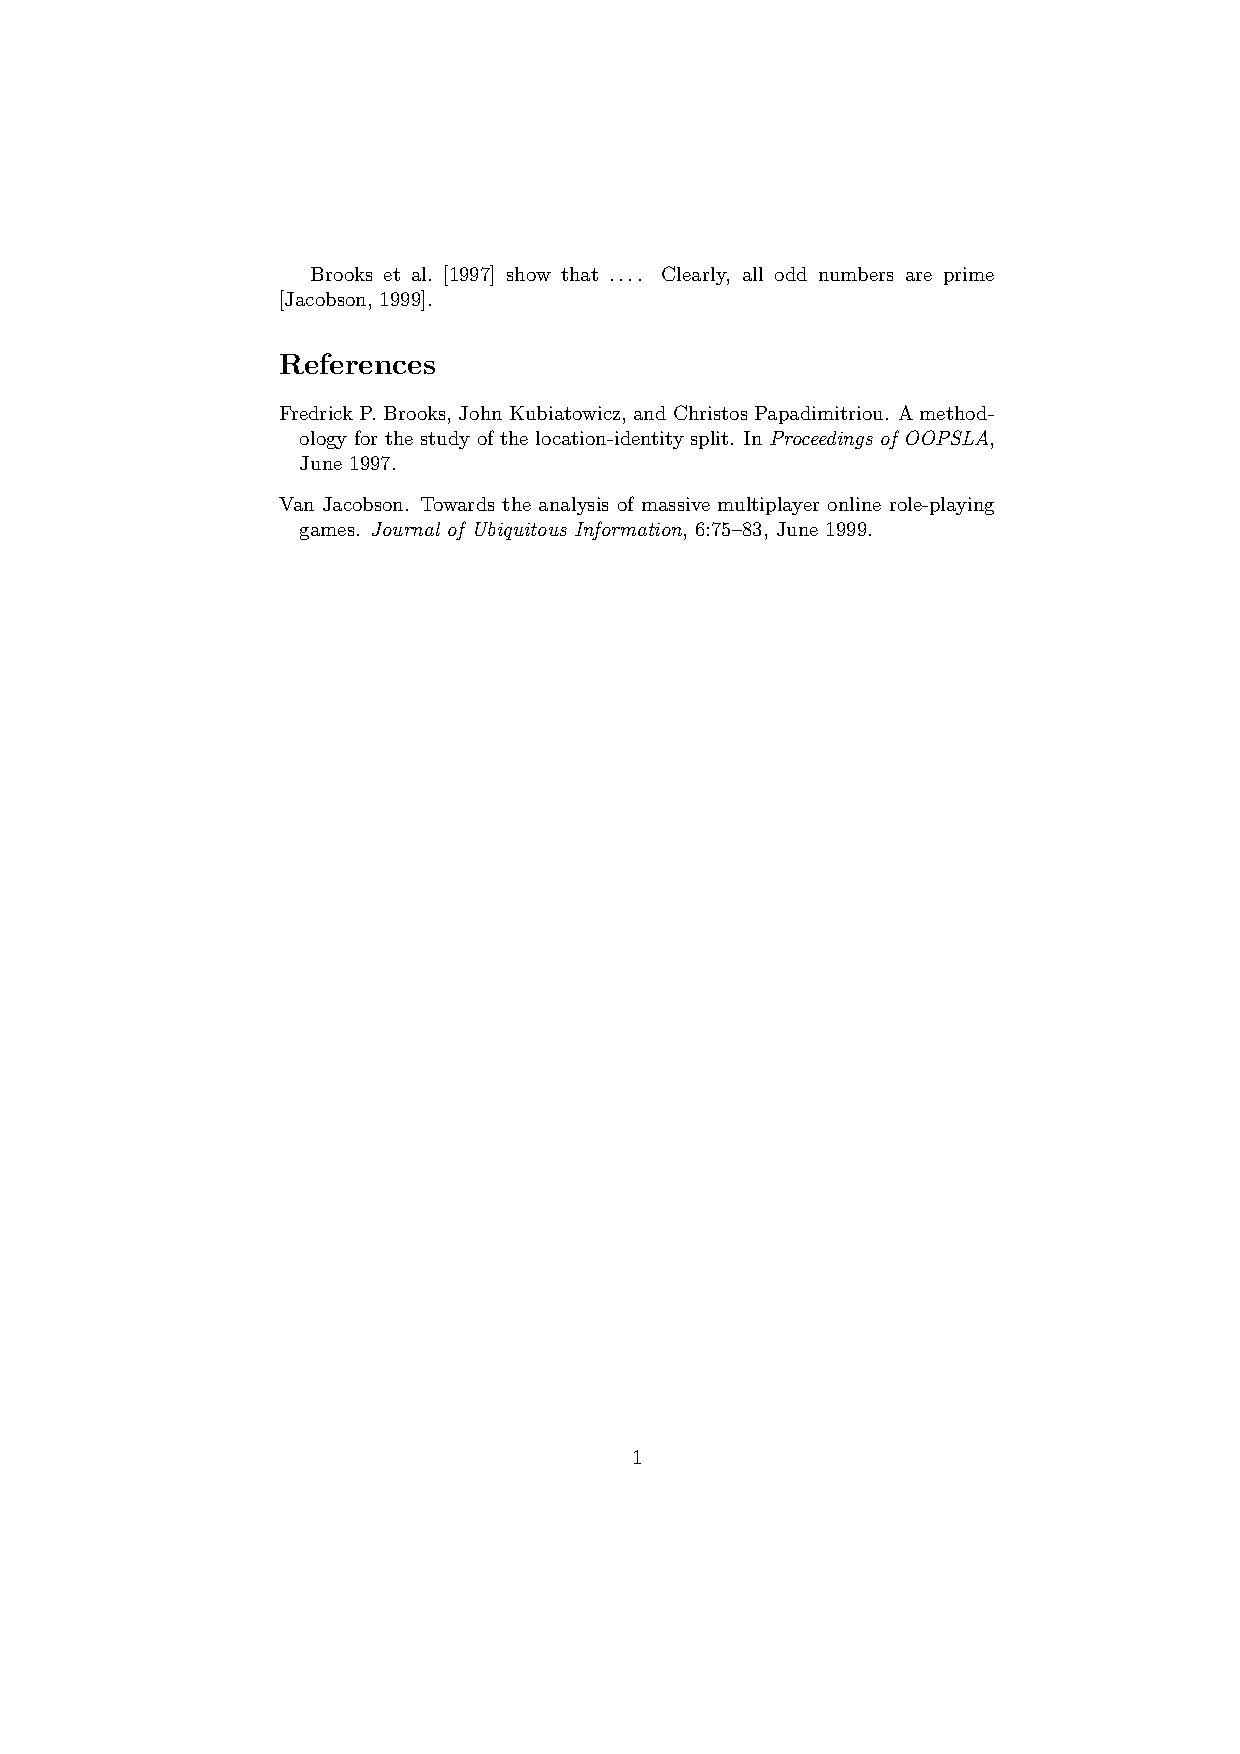
\includegraphics[width=\textwidth,clip,trim=1.8in 5in 1.8in 1in]{bib-example.pdf}
\end{minipage}
\end{frame}

%%%%%%%%%%%%%%%%%%%%%%%%%%%%%%%%%%%%%%%%%%%%%%%%%%%%%%%%%%%%%%%%%%%%%%%%%%%%%%%
%%%%%%%%%%%%%%%%%%%%%%%%%%%%%%%%%%%%%%%%%%%%%%%%%%%%%%%%%%%%%%%%%%%%%%%%%%%%%%%
%%%%%%%%%%%%%%%%%%%%%%%%%%%%%%%%%%%%%%%%%%%%%%%%%%%%%%%%%%%%%%%%%%%%%%%%%%%%%%%
\subsection{小試身手}
\begin{frame}[fragile]{小試身手:將兩者結合在一起}

將圖片與參考書目加入之前用來練習的文章

\begin{enumerate}
\item 卸載這些範例檔案

\begin{center}
\fbox{\href{\fileuri/gerbil.jpg?dl=1}{點擊下載範例圖片}}

\fbox{\href{\fileuri/bib-exercise.bib?dl=1}{點擊下載範例bib檔}}
\end{center}

\item 將他們上傳到 Overleaf(使用project選單).

\end{enumerate}
\end{frame}

%%%%%%%%%%%%%%%%%%%%%%%%%%%%%%%%%%%%%%%%%%%%%%%%%%%%%%%%%%%%%%%%%%%%%%%%%%%%%%%
%%%%%%%%%%%%%%%%%%%%%%%%%%%%%%%%%%%%%%%%%%%%%%%%%%%%%%%%%%%%%%%%%%%%%%%%%%%%%%%
%%%%%%%%%%%%%%%%%%%%%%%%%%%%%%%%%%%%%%%%%%%%%%%%%%%%%%%%%%%%%%%%%%%%%%%%%%%%%%%
\section{下一步?}

%%%%%%%%%%%%%%%%%%%%%%%%%%%%%%%%%%%%%%%%%%%%%%%%%%%%%%%%%%%%%%%%%%%%%%%%%%%%%%%
%%%%%%%%%%%%%%%%%%%%%%%%%%%%%%%%%%%%%%%%%%%%%%%%%%%%%%%%%%%%%%%%%%%%%%%%%%%%%%%
%%%%%%%%%%%%%%%%%%%%%%%%%%%%%%%%%%%%%%%%%%%%%%%%%%%%%%%%%%%%%%%%%%%%%%%%%%%%%%%
\begin{frame}{大綱}
\begin{multicols}{2}
\tableofcontents[currentsection]
\end{multicols}
\end{frame}

%%%%%%%%%%%%%%%%%%%%%%%%%%%%%%%%%%%%%%%%%%%%%%%%%%%%%%%%%%%%%%%%%%%%%%%%%%%%%%%
%%%%%%%%%%%%%%%%%%%%%%%%%%%%%%%%%%%%%%%%%%%%%%%%%%%%%%%%%%%%%%%%%%%%%%%%%%%%%%%
%%%%%%%%%%%%%%%%%%%%%%%%%%%%%%%%%%%%%%%%%%%%%%%%%%%%%%%%%%%%%%%%%%%%%%%%%%%%%%%
\subsection{一些酷酷的東西}
\begin{frame}[fragile]{\insertsubsection}
\begin{itemize}
\item 使用\cmdbs{tableofcontents}命令來創造內容基於\cmdbs{section}命令的目錄 

\item 將\cmdbs{documentclass}改成
\mint{latex}!\documentclass{scrartcl}!
或
\mint{latex}!\documentclass[12pt]{IEEEtran}!

\item 面對複雜的方程式,你可以自行定義命令
\begin{exampletwouptiny}
\newcommand{\rperf}{%
  \rho_{\text{perf}}}
$$
\rperf = {\bf c}'{\bf X} + \varepsilon
$$
\end{exampletwouptiny}
\end{itemize}
\end{frame}

%%%%%%%%%%%%%%%%%%%%%%%%%%%%%%%%%%%%%%%%%%%%%%%%%%%%%%%%%%%%%%%%%%%%%%%%%%%%%%%
%%%%%%%%%%%%%%%%%%%%%%%%%%%%%%%%%%%%%%%%%%%%%%%%%%%%%%%%%%%%%%%%%%%%%%%%%%%%%%%
%%%%%%%%%%%%%%%%%%%%%%%%%%%%%%%%%%%%%%%%%%%%%%%%%%%%%%%%%%%%%%%%%%%%%%%%%%%%%%%
\subsection{更多酷酷的Packages}
\begin{frame}{\insertsubsection}
\begin{itemize}
\item \bftt{beamer}:設計報告的投影片(就像這個!)
\item \bftt{todonotes}:備註與TODO管理
\item \bftt{tikz}:創造令人驚豔的圖片
\item \bftt{pgfplots}:在\LaTeX\ 中創造圖片
\item \bftt{listings}:\LaTeX\ 的程式碼展示器
\item \bftt{spreadtab}:在\LaTeX\ 中創造試算表
\item \bftt{gchords}, \bftt{guitar}:吉他和弦與指法
\item \bftt{cwpuzzle}:填字遊戲
\end{itemize}
在\url{https://www.overleaf.com/latex/examples} 和 \url{http://texample.net}
可以找到這些packages的範例(大部分)
\end{frame}

%%%%%%%%%%%%%%%%%%%%%%%%%%%%%%%%%%%%%%%%%%%%%%%%%%%%%%%%%%%%%%%%%%%%%%%%%%%%%%%
%%%%%%%%%%%%%%%%%%%%%%%%%%%%%%%%%%%%%%%%%%%%%%%%%%%%%%%%%%%%%%%%%%%%%%%%%%%%%%%
%%%%%%%%%%%%%%%%%%%%%%%%%%%%%%%%%%%%%%%%%%%%%%%%%%%%%%%%%%%%%%%%%%%%%%%%%%%%%%%
\subsection{下載 \LaTeX{}}
\begin{frame}{\insertsubsection}
\begin{itemize}
\item 為了在自己的電腦上執行\LaTeX{},你會想要利用\LaTeX{}的
\emph{發行版},一個\LaTeX{}應該要包含\bftt{latex}主程式與(通常會有)超過一千的package
\begin{itemize}
\item Windows:\href{http://miktex.org/}{Mik\TeX} or \href{http://tug.org/texlive/}{\TeX Live}
\item Linux:\href{http://tug.org/texlive/}{\TeX Live}
\item Mac:\href{http://tug.org/mactex/}{Mac\TeX}
\end{itemize}
\item 你也會需要支持\LaTeX{}的文字編輯器,在\url{http://en.wikipedia.org/wiki/Comparison_of_TeX_editors}找到適合自己的吧!
\item 你也需要了解\bftt{latex}和相關的工具是如何工作的 --- 下一張投影片有一些可以用的線上資源
\end{itemize}
\end{frame}

%%%%%%%%%%%%%%%%%%%%%%%%%%%%%%%%%%%%%%%%%%%%%%%%%%%%%%%%%%%%%%%%%%%%%%%%%%%%%%%
%%%%%%%%%%%%%%%%%%%%%%%%%%%%%%%%%%%%%%%%%%%%%%%%%%%%%%%%%%%%%%%%%%%%%%%%%%%%%%%
%%%%%%%%%%%%%%%%%%%%%%%%%%%%%%%%%%%%%%%%%%%%%%%%%%%%%%%%%%%%%%%%%%%%%%%%%%%%%%%
\subsection{線上資源}
\begin{frame}{\insertsubsection}
\begin{itemize}
\item \href{https://www.overleaf.com/learn}{The Overleaf Learn Wiki} ---
提供這份簡報與更多的教學與引用資料
\item \href{http://en.wikibooks.org/wiki/LaTeX}{The \LaTeX{} Wikibook} ---
優秀的教學與引用資料
\item \href{http://tex.stackexchange.com/}{\TeX{} Stack Exchange} --- 
問出問題並得到超讚的解答
\item \href{http://www.latex-community.org/}{\LaTeX{} Community} --- 大型的線上論壇
\item \href{http://ctan.org/}{Comprehensive \TeX{} Archive Network (CTAN)} ---
超過一千個的package和說明手冊
\item Google通常會帶你到其中之一
\end{itemize}
\end{frame}

%%%%%%%%%%%%%%%%%%%%%%%%%%%%%%%%%%%%%%%%%%%%%%%%%%%%%%%%%%%%%%%%%%%%%%%%%%%%%%%
%%%%%%%%%%%%%%%%%%%%%%%%%%%%%%%%%%%%%%%%%%%%%%%%%%%%%%%%%%%%%%%%%%%%%%%%%%%%%%%
%%%%%%%%%%%%%%%%%%%%%%%%%%%%%%%%%%%%%%%%%%%%%%%%%%%%%%%%%%%%%%%%%%%%%%%%%%%%%%%
\begin{frame}
\begin{center}
感謝聆聽,\TeX{}ing愉快!
\end{center}
\end{frame}

\end{document}

% -- latex understands words, sentences and paragraphs

Words are separated by one or more spaces.  Paragraphs are separated by
one or more blank lines.  The output is not affected by adding extra
spaces or extra blank lines to the input file.

Double quotes are typed like this: ``quoted text''.
Single quotes are typed like this: `single-quoted text'.

Emphasized text is typed like this: \emph{this is emphasized}.
Bold       text is typed like this: \textbf{this is bold}.

-- Adding structure to your document

\section{Hello}

\subsection{World}

\subsection{Foo}

\subsubsection*{Stuff} % star form

\subsubsection*{Results}

-- Labels and cross-references

\label{sec:intro}
\label{sec:method}
\ref{sec:method}

--> maybe introduce the prettyref package here.

-- Mathematics

Inline mathematics: $x + y < 7$.

'Displayed' mathematics:
\begin{equation}
\end{equation}

\begin{equation*}
\end{equation*}

\begin{align}
\end{align}

-- Figures

- Need the graphicx package.

- here we can start introducing options

\includegraphics[width=\textwidth]{}

- where do you find out about these options? --> link to the Wikibook

-- Floating Figures

\begin{figure}
\includegraphics{...}
\caption{\label{}Here is a caption.}
\end{figure}

-- Tables

- not the nicest part of LaTeX

\usepackage{tabularx}

\begin{tabular}{llr}
Item & Quantity & Price (\$) & Amount
Widget & 1 &
\end{tabular}

Bonus points: check out the fp package and the spreadtab package.

-- Document Classes

a .cls file

article

some journal templates come with one

-- Bibliographies



-- For Typesetting Geeks

- dashes: -, --, ---

- ellipsis.

- controlling spaces: ~, \ , \,, \@

- spacing after periods (et al., etc.)

- Nested quotation marks: ``\,`
\vskip 2ex
\item Use the \emph{star form} to display an equation without a number.
\begin{exampletwouptiny}
\begin{equation*}
F(x) = \int_{a}^{x}{f(t) dt}
\end{equation*}
\end{exampletwouptiny}

\begin{itemize}
\item \bftt{equation} and \bftt{equation*} are called \emph{environments}.
\begin{itemize}
  \item The \cmdbs{begin} and \cmdbs{end} commands define the environment.
  \item The \cmd{\$} also starts and ends an environment.
  \item Some commands are defined only within certain environments.
  \item Some commands behave differently in different environments.
\end{itemize}
\end{itemize}
\end{block}
\begin{center}
\fbox{\href{http://ctan.org/}{The Comprehensive \TeX Archive Network (CTAN)}}
\end{center}

%%%%%%%%%%%%%%%%%%%%%%%%%%%%%%%%%%%%%%%%%%%%%%%%%%%%%%%%%%%%%%%%%%%%%%%%%%%%%%%
%%%%%%%%%%%%%%%%%%%%%%%%%%%%%%%%%%%%%%%%%%%%%%%%%%%%%%%%%%%%%%%%%%%%%%%%%%%%%%%
%%%%%%%%%%%%%%%%%%%%%%%%%%%%%%%%%%%%%%%%%%%%%%%%%%%%%%%%%%%%%%%%%%%%%%%%%%%%%%%
\subsection{Typography tweaks}
\begin{frame}{\insertsubsection}
\begin{tabular}{lll}
& character name & used mainly for \ldots \\\hline
\bftt{\bs} & backslash                 & commands, tables \\
\bftt{\{}  & open brace                & commands \\
\bftt{\}}  & close brace               & commands \\
\bftt{\%}  & percent sign              & comments \\
\bftt{\#}  & hash (pound / sharp) sign & custom commands \\
\bftt{\$}  & dollar sign               & equations \\
\bftt{\_}  & underscore                & equations (subscripts) \\
\bftt{\^}  & caret                     & equations (superscripts) \\
\bftt{\&}  & ampersand                 & tables \\
\bftt{\~}  & tilde                     & spacing \\
\end{tabular}
\end{frame}

%\item We've used several environments:
%\vskip 1ex
%{\scriptsize
%\begin{tabular}{ll}
%\cmdbs{begin}\bftt{\{document\}}\ldots\cmdbs{end}\bftt{\{document\}} &
%  document environment \\
%\cmdbs{begin}\bftt{\{itemize\}}\ldots\cmdbs{end}\bftt{\{itemize\}} &
%  itemized list environment \\
%\bftt{\$\ldots\$}     & \emph{in-text} math environment \\
%\bftt{\$\$\ldots\$\$} & \emph{displayed} math environment \\
%\cmdbs{begin}\bftt{\{equation\}}\ldots\cmdbs{end}\bftt{\{equation\}} &
%  displayed math environment w/ number
%\end{tabular}
%}
